\documentclass[../EBEXPaper2.tex]{subfiles}
\begin{document}
%------------------------------------------------- 
\subsubsection{Optical Efficiency}
\label{sec:optical_efficiency}

\begin{itemize}
\item \comred{Francois in charge}
\end{itemize}

The total optical efficiency of the \ac{EBEX} telescope $\epsilon_{telescope}$ is the product of the transmission of its optical elements $\tau_{optical}$ and the detector absorption efficiency $\epsilon_{bolo}$:
\begin{equation}
\epsilon_{telescope} = \tau_{optical} \epsilon_{bolo}.
\label{eq:total_efficiency}
\end{equation}
The  transmission of the optical elements is the product of the transmission of each of the optical elements
\begin{equation}
\tau_{optical} = \prod_i \tau_i,
\label{eq:total_efficiency}
\end{equation}
where $\tau_i$ is the transmission of the $i^{th}$ optical element.
The transmission of each optical element is calculated from first principles as described in \citep{aubin_thesis}.
In this section, we utilize the calculations of $\tau_{optical}$ and the measurements of the optical efficiency of the telescope $\epsilon_{telescope}$ performed on the ground before the \ac{EBEX2013} flight and at float during the \ac{EBEX2013} flight to measure the absorption efficiency of the \ac{EBEX} bolometers.


\subsubsubsection{Lab Measurements}

We measure the absorption efficiency of the bolometers populating one bolometer wafer fabricated to observe within each of the three \ac{EBEX} frequency bands.
These detectors are operated inside the \ac{EBEX} cryostat on which a blackbody source is mounted, replacing the cryostat window.
We set and measure the temperature of the blackbody source $T_{BB}$.
We calculate its emitted power $P_{BB}^{band} (T_{BB})$ by integrating the blackbody spectrum over each of the three \ac{EBEX} frequency bands.
We then measure the saturation power of the detectors exposed to the blackbody as a function of $T_{BB}$.
We use the ``dark'' saturation power of each bolometer to measure the optical power $P_{rad}$ they absorbe following the methodology described in Section~\ref{sec:optical_load}.
We have previously characterized the ``dark'' saturation power by measuring the saturation power of the bolometers in a cryostat closed to external light at various bath temperatures as described in \citep{Aubin_TESReadout2010}.
The left panel of Figure~\ref{fig:efficiency} shows such a measurement for the representative bolometer 150-G17-05-05.
We fit for the amplitude of the ratio between $P_{BB}^{band}$ and $P_{rad}$ to extract $\epsilon_{telescope}$.

\begin{figure}[htbp]
\centering
% \leavevmode
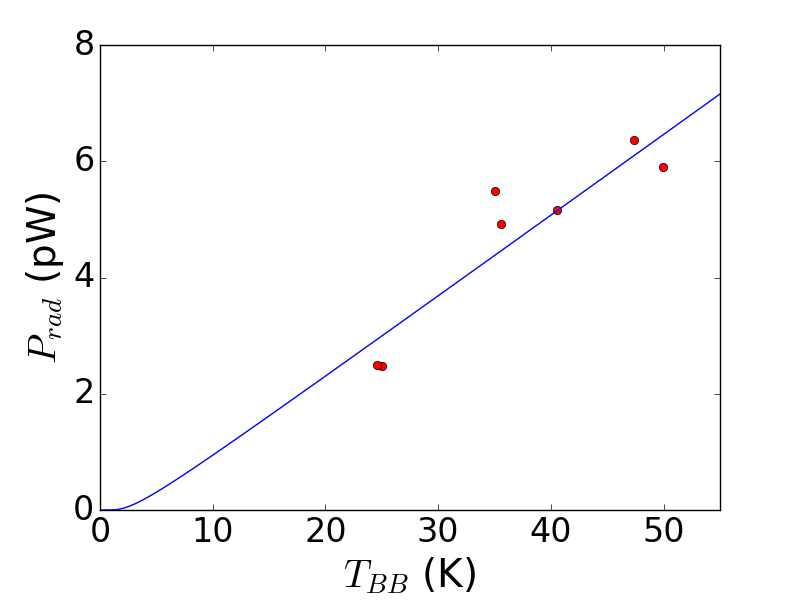
\includegraphics[height={5.5cm}]{images/detectors_and_readout/150-05-05}%
\hfil
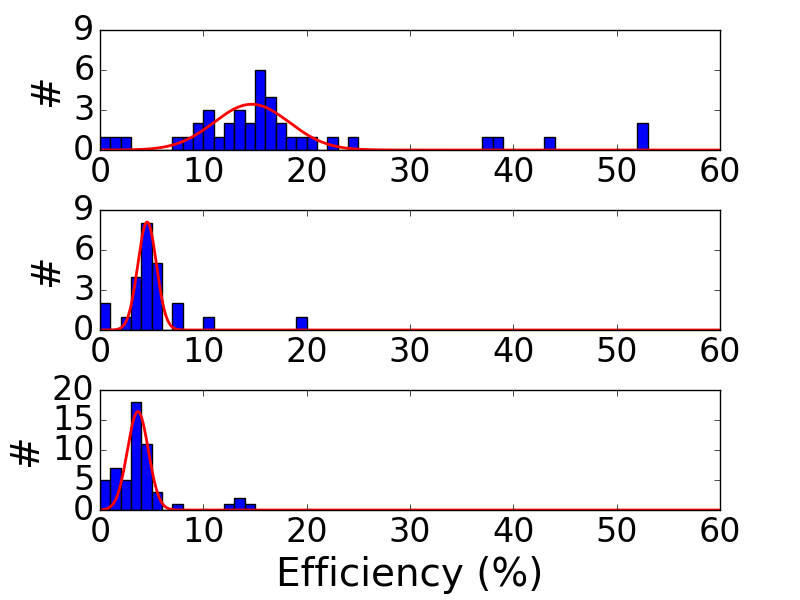
\includegraphics[height={5.5cm}]{images/detectors_and_readout/hist_efficiency_BB}%
\caption{Left panel: The measured (red circles) and fitted (solid line) power absorbed by bolometer 150-G17-05-05 as a function of the blackbody temperature.
The total telescope efficiency is fitted to 16\%.%15.6
Right panel: The distribution of the total telescope efficiency for bolometer wafers 150-G17 (upper pannel), 250-G20 (middle panel), and 410-G18 (lower panel).
The distributions are fitted to Gaussian functions (red solid line) with averages and standard deviations of (15 $\pm$ 4)\%, (4.6 $\pm$ 0.9)\%, and (4 $\pm$ 1)\%, respectively.%(14.7 $\pm$ 3.6)\%, (4.6 $\pm$ 0.9)\%, and (3.7 $\pm$ 1.0)\%
}
\label{fig:efficiency}
\end{figure}

The right panel of Figure~\ref{fig:efficiency} shows the distributions of the total telescope efficiencies for the three \ac{EBEX} frequency bands.
We include all bolometers reliably dropped in their superconducting transition.
We characterize the distributions by fitted Gaussian function with averages of 15, 4.6, and 4\% and a standard deviations of 4, 0.9, and 1\% for the 150, 250, and 410~GHz detectors, respectively.
The width of these distributions is caused by the variability of the fabrication parameters.
The bolometer absorption efficiency is derived from Equation~\ref{eq:total_efficiency} using the fitted telecope efficiency for each detector and the transmission of the optical elements of the telescope shown in Table~\ref{tab:transmissions}.
The average bolometer absorption efficiency is 80, 28, and 27\% with a standard deviation of 20, 6, and 7\% for the 150, 250, and 410~GHz detectors, respectively.%76.6, 28.4, and 27.0\% with a standard deviation of 18.8, 5.6, and 7.3\%

%%%%%%%%%%%%%%%%%%%%%%%%%%%%%%%%%%%%%%%%
\begin{table}[htbp]
\caption{Transmission of each optical element within the \ac{EBEX} cryostat for the bolometer absorption efficiency measured on the ground before the \ac{EBEX2013} flight and during the \ac{EBEX2013} flight.}
\begin{center}
\setlength\tabcolsep{3.0pt}
\begin{tabular}{|l||c|c|c||c|c|c|}
\multicolumn{4}{l}{} \\ \hline
& \multicolumn{3}{|c||}{Pre-EBEX2013} & \multicolumn{3}{|c|}{EBEX2013} \\ \hline
Optical element & 150 GHz & 250 GHz & 410 GHz & 150 GHz & 250 GHz & 410 GHz \\ \hline \hline
Primary mirror & N/A & N/A & N/A & 1.00 & 1.00 & 1.00 \\ \hline
Secondary mirror & N/A & N/A & N/A & 1.00 & 1.00 & 1.00 \\ \hline
Cryostat window & N/A & N/A & N/A & 0.97 & 0.96 & 0.97 \\ \hline
Teflon filter  & 0.92 & 0.89 & 0.84 & 0.95 & 0.93 & 0.88 \\ \hline
LPE1 filter    & 0.99 & 0.95 & 0.98 & 0.98 & 0.98 & 0.97 \\ \hline
LPE2 filter    & 0.95 & 0.96 & 0.98 & 0.98 & 0.98 & 0.96 \\ \hline
LPE3 filter    & 0.96 & 0.97 & 0.95 & N/A & N/A & N/A \\ \hline
LPE4 filter    & 0.96 & 0.90 & 0.91 & N/A & N/A & N/A \\ \hline
Field lens     & 0.92 & 0.91 & 0.89 & 0.96 & 0.93 & 0.83 \\ \hline
LPE2b filter  & 0.98 & 0.99 & 0.90 & 0.98 & 0.97 & 0.96 \\ \hline
HWP             & 0.54 & 0.53 & 0.52 & 0.94 & 0.93 & 0.91 \\ \hline
Pupil lens 1  & 1.00 & 0.99 & 0.98 & 0.97 & 0.93 & 0.90 \\ \hline
Pupil lens 2  & 1.00 & 0.99 & 0.98 & 0.97 & 0.93 & 0.90 \\ \hline
Polarizing grid & 0.50 & 0.50 & 0.50 & 0.50 & 0.50 & 0.50 \\ \hline
Camera lens & 0.99 & 0.98 & 0.96 & 0.97 & 0.94 & 0.91 \\ \hline \hline
Total            & 0.19 & 0.16 & 0.14 & 0.35 & 0.28 & 0.21 \\ \hline
\end{tabular}
\end{center}
\label{tab:transmissions}
\end{table}
%%%%%%%%%%%%%%%%%%%%%%%%%%%%%%%%%%%%%%%%

% %%%%%%%%%%%%%%%%%%%%%%%%%%%%%%%%%%%%%%%%
% \begin{table}[htbp]
% \caption{Transmission of each optical element within the EBEX cryostat for the bolometer absorption efficiency measured on the ground before the \ac{EBEX2013} flight.}
% \begin{center}
% \begin{tabular}{|l|c|c|c|}
% \multicolumn{4}{l}{} \\ \hline
% Optical element & 150 GHz & 250 GHz & 410 GHz \\ \hline
% Teflon filter  & 0.92 & 0.89 & 0.84 \\ \hline
% LPE1 filter    & 0.99 & 0.95 & 0.98 \\ \hline
% LPE2 filter    & 0.95 & 0.96 & 0.98 \\ \hline
% LPE3 filter    & 0.96 & 0.97 & 0.95 \\ \hline
% LPE4 filter    & 0.96 & 0.90 & 0.91 \\ \hline
% Field lens     & 0.92 & 0.91 & 0.89 \\ \hline
% LPE2b filter  & 0.98 & 0.99 & 0.90 \\ \hline
% HWP             & 0.54 & 0.53 & 0.52 \\ \hline
% Pupil lens 1  & 1.00 & 0.99 & 0.98 \\ \hline
% Pupil lens 2  & 1.00 & 0.99 & 0.98 \\ \hline
% Polarizing grid & 0.50 & 0.50 & 0.50 \\ \hline
% Camera lens & 0.99 & 0.98 & 0.96 \\ \hline \hline
% $\tau_{optical}$ & 0.19 & 0.16 & 0.14 \\ \hline
% \end{tabular}
% \end{center}
% \label{tab:transmissions_run8}
% \end{table}
% %%%%%%%%%%%%%%%%%%%%%%%%%%%%%%%%%%%%%%%%


\subsubsubsection{At Float Measurements}

During the \ac{EBEX2013} flight, we calibrated the response of the \ac{EBEX} bolometers to the Galactic plane as described in \citep{Aubin_MGrossman2015}.
The calibration factor $\frac{d P_{sky}^W}{d I_{bolo}^{counts}}$ provides the conversion from current flowing through the TES bolometer in raw readout units to power on the sky for each detector.
The calibration factor is converted to the bolometer absorption efficiency, which is the ratio between the power absorbed by the bolometer to the power incident on the bolometer, following
\begin{equation}
\epsilon_{bolo} = \frac{ S_I \times \frac{d I_{bolo}^A}{d I_{bolo}^{counts}}}{ \tau_{optical}} \left( \frac{d I_{bolo}^{counts}}{d P_{sky}^W} \right),
\label{eq:bolo_efficiency_form_calib}
\end{equation}
where $\frac{d I_{bolo}^A}{d I_{bolo}^{counts}}$ is the transfer function of the DfMUX readout boards and $S_I \equiv \frac{d P_{bolo}^W}{d I_{bolo}^A}$ is the bolometer responsivity.
The transfer function of the readout boards converts the current flowing through the TES bolometer from raw readout units to Ampere and the responsivity converts this current to power absorbed by the bolometer.
Both quantities are derived in \citep{aubin_thesis}.
The total transmission of the telescope $\tau_{optical}$ during the \ac{EBEX2013} flight is shown in Table~\ref{tab:transmissions} and converts the power on the sky to incident power on the bolometers.

% \begin{table}[htbp]
% \caption{Transmission coefficients of the different optical elements in the \ac{EBEX} cryostat to a single focal plane for the \ac{EBEX2013} flight within the 150, 250, and 410 GHz observing frequency bands calculated from first principles.}
% \begin{center}
% \begin{tabular}{|l|c|c|c|}
% \multicolumn{4}{l}{} \\ \hline
% Optical element & 150 GHz & 250 GHz & 410 GHz \\ \hline
% Primary mirror & 1.00 & 1.00 & 1.00 \\ \hline
% Secondary mirror & 1.00 & 1.00 & 1.00 \\ \hline
% Cryostat window & 0.97 & 0.96 & 0.97 \\ \hline
% Teflon filter  & 0.95 & 0.93 & 0.88 \\ \hline
% LPE1 filter    & 0.98 & 0.98 & 0.97 \\ \hline
% LPE2 filter    & 0.98 & 0.98 & 0.96 \\ \hline
% Field lens     & 0.96 & 0.93 & 0.83 \\ \hline
% LPE2b filter  & 0.98 & 0.97 & 0.96 \\ \hline
% HWP             & 0.94 & 0.93 & 0.91 \\ \hline
% Pupil lens 1  & 0.97 & 0.93 & 0.90 \\ \hline
% Pupil lens 2  & 0.97 & 0.93 & 0.90 \\ \hline
% Polarizing grid & 0.50 & 0.50 & 0.50 \\ \hline
% Camera lens & 0.97 & 0.94 & 0.91 \\ \hline \hline
% Total            & 0.35 & 0.28 & 0.21 \\ \hline
% \end{tabular}
% \end{center}
% \label{tab:transmissions_ebex2013}
% \end{table}

Figure~\ref{fig:opt_eff_from_calib_dist} shows the distributions of the bolometer absorption efficiencies per frequency band.
The distributions for the 150, 250, and 410~GHz bolometers are fitted to Gaussian functions and have an average of 29, 20, and 2.6\% and a standard deviation of 6, 10, and 0.9\%, respectively. %28.6, 22.0, and 2.6\% and a standard deviation of 6.1, 11.3, and 0.9\%
\comred{The conclusions need to be double-checked. The ground measurements show 80, 30, 30\%; this section shows 30, 20, 3\% and the measurements of the load at float (Section~\ref{sec:optical_load}) show 80, 70 and 40\%.}

\begin{figure}[htbp]
\centering
% \leavevmode
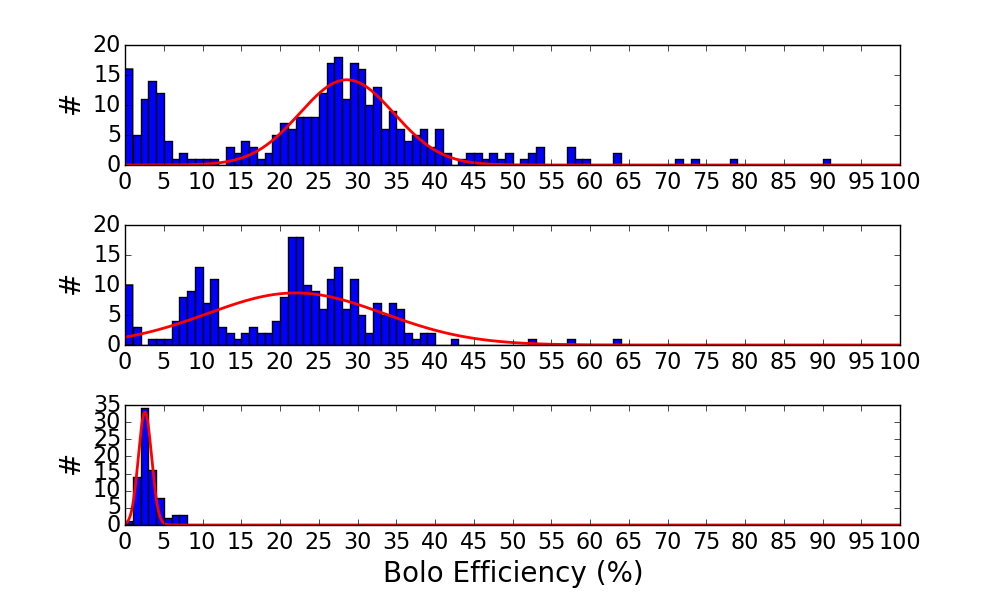
\includegraphics[height={6.5cm}]{images/detectors_and_readout/opt_eff_from_calib_dist}%
\caption{The measured and fitted (red solid line) bolometer absorption efficiency extracted from the \ac{EBEX2013} flight bolometer calibration for the 150 (upper panel), 250 (middle panel), and 410~GHz (lower panel) frequency band.
The distributions are fitted to Gaussian functions with averages and standard deviations of (29 $\pm$ 6)\%, (20 $\pm$ 10)\%, and (2.6 $\pm$ 0.9)\%, respectively.%(28.6 $\pm$ 6.1)\%, (22.0 $\pm$ 11.3)\% and (2.6 $\pm$ 0.9)\%
}
\label{fig:opt_eff_from_calib_dist}
\end{figure}

\comred{Add a paragraph about expectations and how the data fits to these expectations. FA}


%------------------------------------------------
%\include{DetectorReadoutBibliography}
\end{document}
